\chapter{Knihovna GEOC}
\label{5-geoc}

\section{Tvorba knihovny GEOC}
\label{knihovna}

Algoritmy týkající se slučování vektorových map (\textit{conflation}) byly
implementovány v~externí knihovně \textit{GEOC} bez závislosti na~QGIS API. 
Zásuvný modul \textit{Conflate} umožňuje využití funkcionality knihovny 
v~Quantum GIS. Díky tomuto oddělení vznikla nezávislá knihovna, kterou bude
možné případně použít i~v~jiných programech a~projektech.

Tato kapitola popisuje jednotlivé algoritmy a~jejich implementaci v~knihovně
\textit{GEOC}, zároveň také stručně pojednává o~možnostech  jejich využití.
Podrobný popis jednotlivých tříd a~jejich metod je podrobněji popsán v~dokumentaci. % viz příloha

% úvodní poznámky, proč samost. knihovna (aby se to dalo využít i jinde než v mém pluginu)
% co popisuje kapitola, vyjmenování algoritmů, jakou funkcionalitu by měla zajišťovat (stručně)

\section{Vertex Snapper} 
\label{vertexsnapper}

Při zpracování vrstev z~více zdrojů někdy stačí pouze upřesnit polohu či tvar 
prvků z~cílové vrstvy tak, aby se přiblížil prvkům z~vrstvy referenční. 
\mbox{Není-li} podrobnost obou datasetů příliš rozdílná, lze využít jednoduchého 
postupu \textbf{přichycení blízkých vrcholů}.

\subsection{Popis algoritmu}
\label{vs-algoritmus}

Nejjednodušším způsobem kombinace dvou vektorových vrstev je pouhé přichycení 
blízkých vrcholů cílové vrstvy k~vrstvě referenční. Obecný postup je následující:

\begin{enumerate}
 \item Na~počátku je třeba určit vzdálenostní toleranci, tedy maximální 
    vzdálenost mezi~dvěma body, kdy ještě bude provedeno jejich přichycení.
 \item Ke~každému prvku ze~zpracovávané vrstvy nalezneme nejbližší prvky 
    z~vrstvy referenční. To jsou prvky, jejichž nejkratší vzdálenost 
    od~zpracovávaného prvku není větší	než vzdálenostní tolerance.
 \item Pro~každý bod ze~zpracovávaného prvku vypočteme vzdálenosti ke~všem
    bodům z~blízkých referenčních prvků.
 \item Pokud nejmenší z~těchto délek je menší než vzdálenostní tolerance, 
    pak posuneme zpracovávaný bod do~odpovídajícího referenčního bodu s~touto
    nejmenší vzdáleností.
 \item Takto projdeme postupně všechny vrcholy všech prvků cílové vrstvy 
    a~snažíme se k~nim nalézt blízké body z~prvků vrstvy referenční. 
\end{enumerate}

% obrázek ilustrujici postup zpracovani
\label{vspic}
  \begin{figure}[hbt]
    \centering
      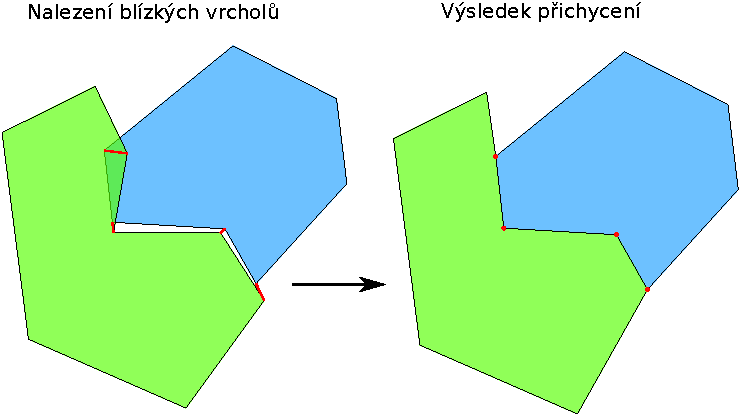
\includegraphics[width=300pt]{./pictures/vs-princip.pdf}
      \caption{Postup přichycení vrcholů (\todo{zdroj})}
      \label{fig:vs-princip}
  \end{figure}

\subsection{Implementace} % text asi přepsat 
\label{vs-implementace}
% popis mé implementace algoritmu + zmínit třídy a funkce s odkazy na literaturu
Algoritmus pro~přichycení vrcholů upravované vrstvy k~referenční je 
implementován ve~třídách \texttt{Vertex\-Snapper} 
a~\texttt{Vertex\-Geometry\-Editor\-Operation}. Při~použití v~externí aplikaci 
stačí po~předání vstupních parametrů třídě \texttt{Vertex\-Snapper} zavolat 
funkci \texttt{snap}. Ta vyhledá blízké prvky s~využitím prostorových 
indexů sestavených metodou \texttt{build\-Index} téže třídy.

Výsledky vyhledávání poté předá funkci \texttt{snap\-Vertices}. Uvnitř této
metody se vytvoří instance  třídy \texttt{Vertex\-Geometry\-Editor\-Operation},
která edituje příslušnou geometrii přichycením blízkých vrcholů.
\texttt{Vertex\-Geometry\-Editor\-Operation} je potomkem třídy 
\texttt{geos::\-operation::\-Coordinate\-Operation}, která je \textit{inter\-face}
\footnote{rozhraní třídy, kde jsou deklarovány pouze abstraktní metody bez
implementace, není možné vytvořit instanci této třídy} třídou pro editaci 
geometrie.


\subsection{Využití}
\label{vs-vyuziti}

Přichycení bodů jedné vrstvy k~vrstvě druhé má své výhody i~nevýhody, které 
je před volbou tohoto způsobu zpracování třeba zvážit. Použití této metody 
je vhodné v~takových případech, kdy máme k~dispozici dvě vrstvy o~rozdílné 
přesnosti (tento rozdíl však nesmí být příliš veliký) a~prvky vzájemně se 
překrývající. Cílem je upřesnit polohu a~tvar prvků z~méně přesného datasetu. 
Dopředu je třeba si uvědomit, že kromě polohy prvků je měněn i~jejich tvar.

Využít by tento postup šel i~pro~přichycení dvou sousedních vrstev o~stejné 
přesnosti, avšak to znamená, že by se změnil pouze tvar krajních prvků 
(nedošlo by k~posunu celé vrstvy), a~to nemusí být vždy žádoucí. Jako jediný
z~algoritmů \textit{GEOC} má pak smysl pro~bodové vrstvy.

Pro~rozumné výsledky je důležité zvolit vhodnou toleranční vzdálenost. Tato 
hodnota by měla odpovídat maximální vzdálenosti, o~kterou se vrchol prvku 
může posunout. Při~volbě příliš krátké vzdálenosti se výsledná vrstva nemusí 
vůbec odlišovat od té vstupní. Naopak \mbox{je-li} zvolená vzdálenost delší 
než nejkratší úsek geometrie (linie, polygonu), může dojít k~přichycení dvou 
bodů k~jednomu bodu z~referenční vrstvy. Zda je toto přípustné či nikoli je 
už na~rozhodnutí uživatele.

\label{vsinvalid}
  \begin{figure}[hbt]
    \centering
      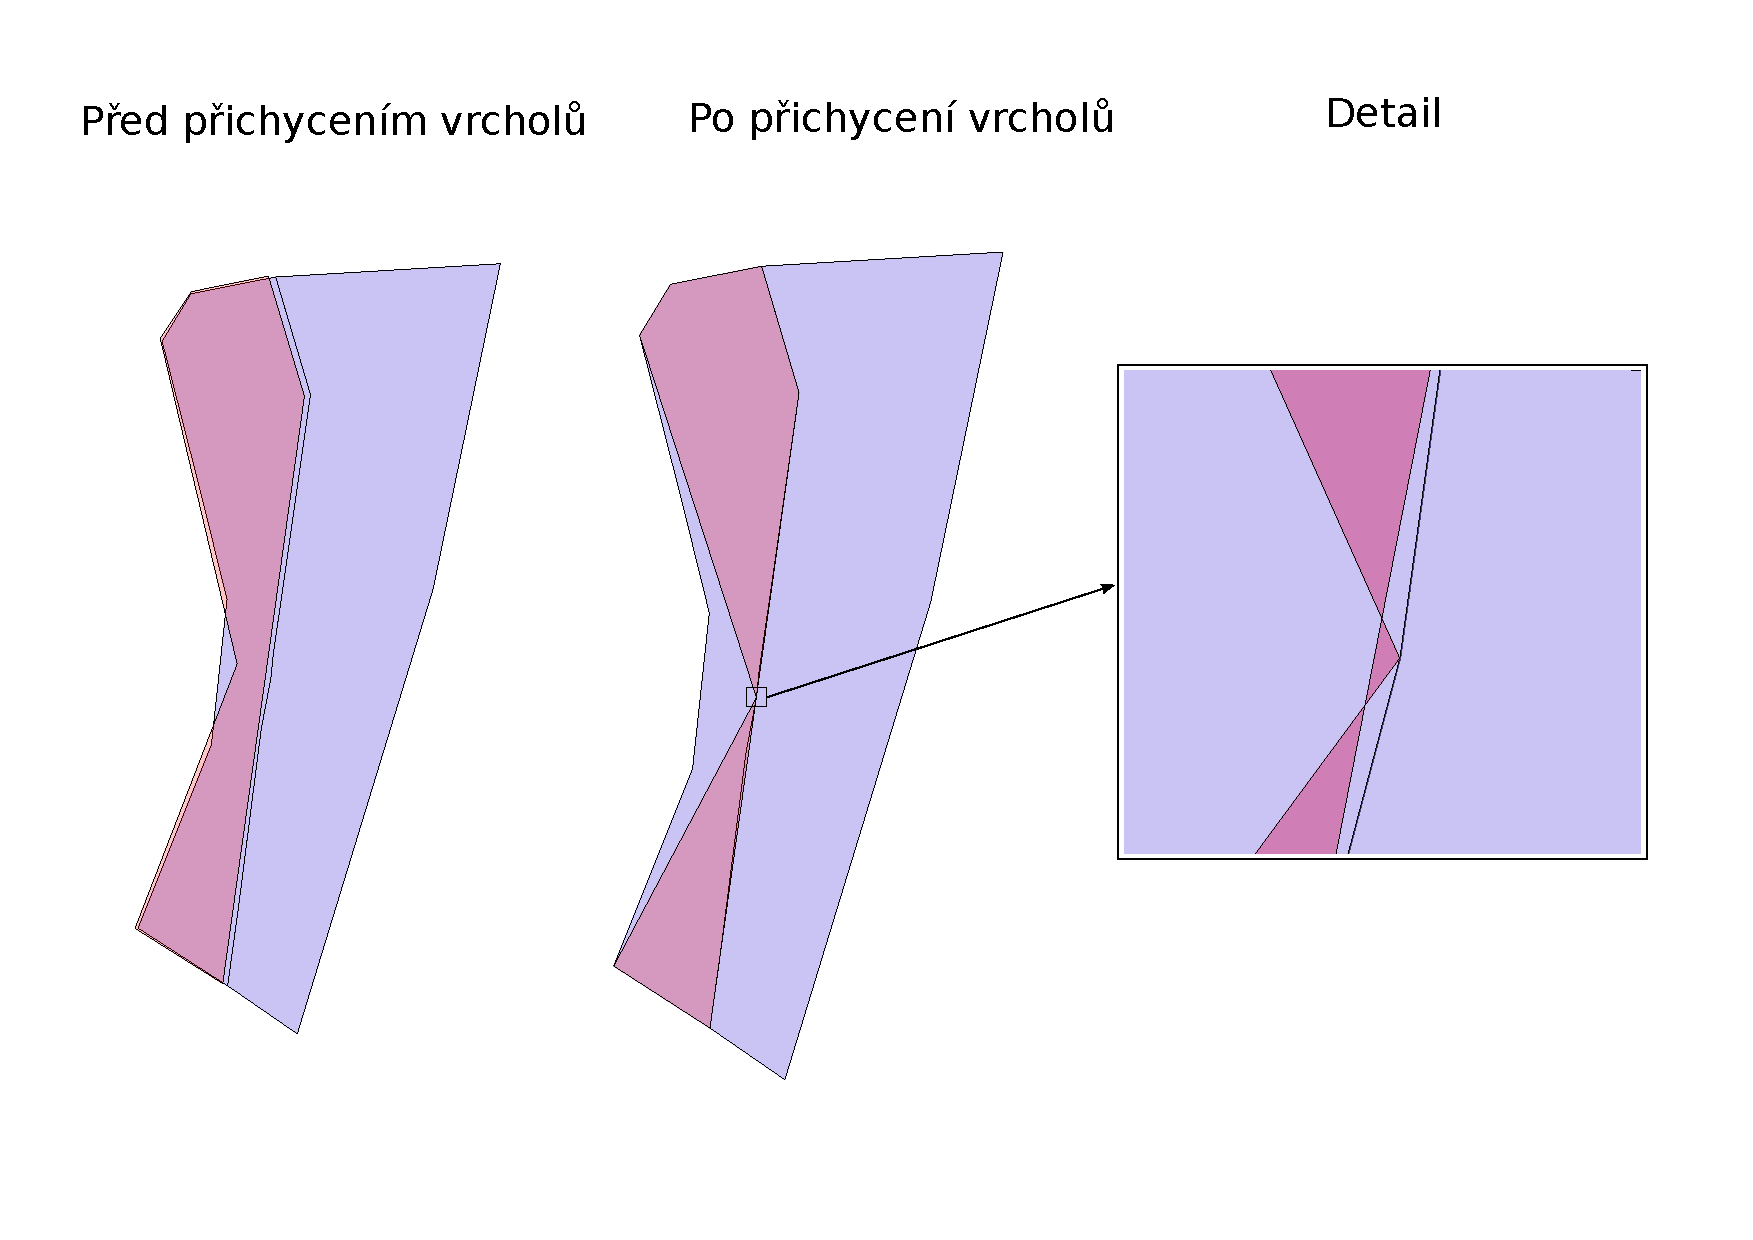
\includegraphics[width=350pt]{./pictures/vs-invalid.pdf}
      \caption{Vznik nevalidní geometrie při přichycení vrcholů (\todo{zdroj})}
      \label{fig:vs-nevalidni}
  \end{figure} 

V~některých případech může dojít ke~vzniku nevalidních geometrií, to je takových,
jejichž segmenty se vzájemně protínají apod. To se nejčastěji stává u~protáhlých 
úzkých prvků a~jiných speciálních tvarů. Příkladem může být situace uvedená 
na~obrázku \ref{fig:vs-nevalidni}, kde růžový polygon je prvkem přichycen 
k~referenční fialové vrstvě, ale z~důvodu nedostatečné hustoty vrcholů a~nevhodného
tvaru vzniká nežádoucí křížení. 


%Někdy může být tento postup výhodný i~v~případě, kdy chceme odstranit drobné mezery či 
%překryty v~rámci jedné vrstvy. Poté stačí nastavit danou vrstvu jako referenční i~jako
%cílovou.  -- teď to ale nejde, protože se z mezer stanou překryty apod. (vrstva se v 
%průběhu nemění), ale šlo by to asi dodělat. 


\section{Coverage Alignment} 
\label{coverage alignment}

\textit{Coverage alignment} lze vysvětlit jako \textbf{zarovnání jedné vrstvy 
k~vrstvě druhé}. Tento způsob je složitější než výše uvedené přichytávání vrcholů.
V~knihovně \textit{GEOC} je využit opět pro~úpravu jedné vrstvy na~základě vrstvy 
referenční. Do~upravované vrstvy nejsou žádné prvky přidávány ani z~ní vymazávány,
pouze jde o~jejich modifikaci. Velmi podobný algoritmus se však dá použít 
i~ke~kombinaci dvou vrstev. 

\subsection{Popis algoritmu}
\label{ca-algoritmus}

Nejčastější používaný postup při~spojování vektorových map je následující.

\begin{enumerate}
 \item Nejprve je třeba nalézt odpovídající si prvky v~obou překrývajících se 
    vrstvách. Kritéria pro~určení odpovídajících si prvků mohou být velmi 
    odlišná. Existuje mnoho algoritmů řešících tuto problematiku, přičemž 
    postupy se mohou různit podle toho, zda je úkolem vyhledání 
    odpovídajících si bodů, polygonů či linií. Kritéria a~postup použitý 
    v~knihovně \textit{GEOC} je popsán níže.
 \item Poté, co se určí odpovídající si prvky, musí se určit totožné vrcholy 
    těchto dvojic prvků. Ty z~vrcholů, které jsou určeny s~dostatečnou 
    přesností (ta může být určena například danou vzdálenostní tolerancí), 
    jsou označeny jako body budoucí triangulační sítě.
 \item Jak už bylo naznačeno, z~nalezených bodů se vytvoří pomocí Delaunayho 
    triangulace\footnote{Delaunayho triangulace z~množiny bodů v~rovině vytvoří takovou 
    trojúhelníkovou síť, pro kterou platí, že v~kružnici opsané každému
    trojúhelníku, neleží žádný jiný bod. DT maximalizuje
    minimální úhly trojúhelníků.} trojúhelníková síť. 
    %ML: doplnit poznamku pod carou - kratka charakteristka DT .. doplneno
 \item Následně se provede lokální, nejčastěji afinní transformace v~každém 
    trojúhelníku sítě. Tak se přetransformují body cílové vrstvy do~systému 
    vrstvy referenční.
 \item Celý postup je možné iterativně opakovat, dokud nedosáhneme 
    požadovaného výsledku (ten může být dán např. podmínkou minimálního 
    množství nalezených odpovídajících si vrcholů či prvků).
\end{enumerate}

% obrázek ilustrujici postup zpracovani, vč. tinu apod.
\label{capic}
  \begin{figure}[hbt]
    \centering
      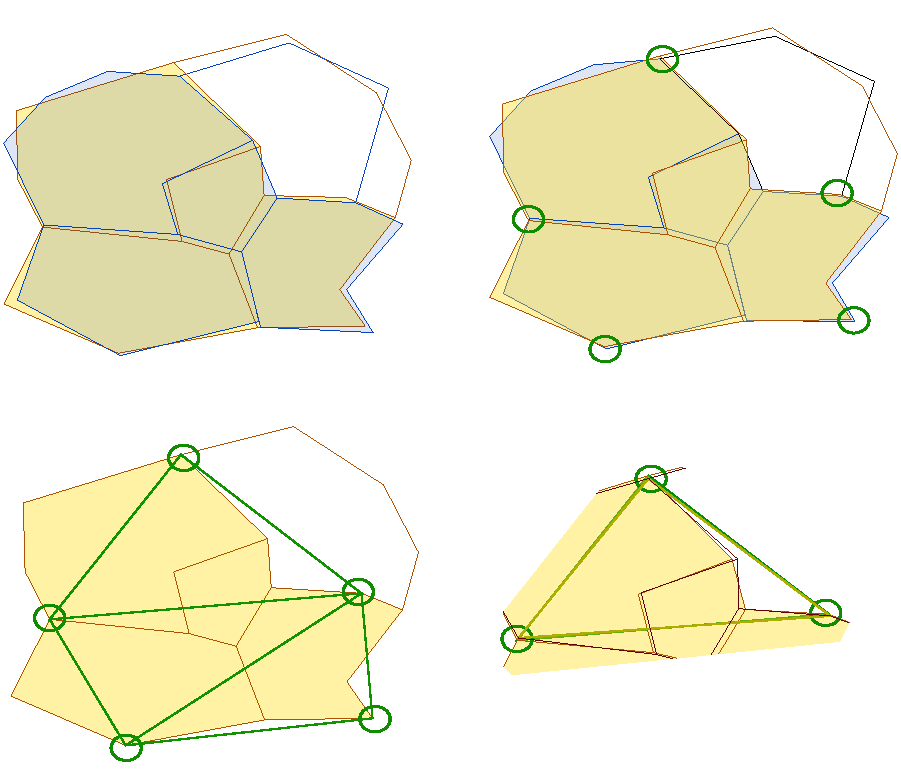
\includegraphics[width=350pt]{./pictures/ca-princip.pdf}
      \caption{Postup zarovnání vrstev (\todo{zdroj})}
      \label{fig:ca-princip}
  \end{figure}

V~knihovně \textit{GEOC} je pro nalezení odpovídajících si prvků využito 
obdobného postupu jako ve~výše zmiňované knihovně \textit{JCS}. Využívá 
se vrcholová Hausdorffova vzdálenost, přičemž tato vzdálenost není počítána 
přímo. Splnění podmínky, že dané prvky nejsou od~sebe dále, než je daná 
Hausdorffova vzdálenost, se testuje pomocí obalových zón jednotlivých prvků 
následujícím způsobem.

\begin{enumerate}
 \item Máme dva prvky A a~B ze~dvou různých překrývajících se vrstev.
 \item Pokud prvek B leží v~obalové zóně prvku A o~velikosti vzdálenostní 
    tolerance a~A leží v~obalové zóně prvku B o~stejné velikosti, je možné, 
    že si prvky odpovídají a~pokračuje se dalším krokem. Situace je naznačena
    na~obrázku \ref{fig:buffer}. V~opačném případě si prvky neodpovídají.

\label{bfpic}
  \begin{figure}[hbt]
    \centering
      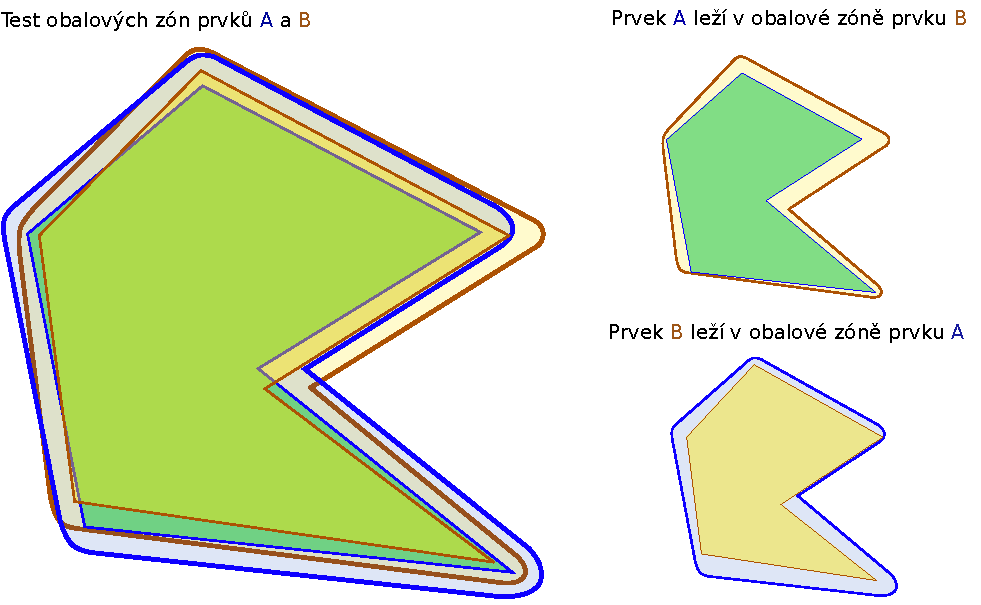
\includegraphics[width=300pt]{./pictures/buffer-test.pdf}
      \caption{Porovnání prvků na základě jejich obalových zón (\todo{zdroj})}
      \label{fig:buffer}

  \end{figure}
 \item Dále se testuje, zda hranice prvku B leží v~obalové zóně hranice prvku
    A a~naopak (viz obrázek \ref{fig:buffer-boundary}). Je-li splněna i~tato 
    podmínka, pak jsou prvky označeny za~odpovídající si.

\label{bf2pic}
  \begin{figure}[hbt]
    \centering
      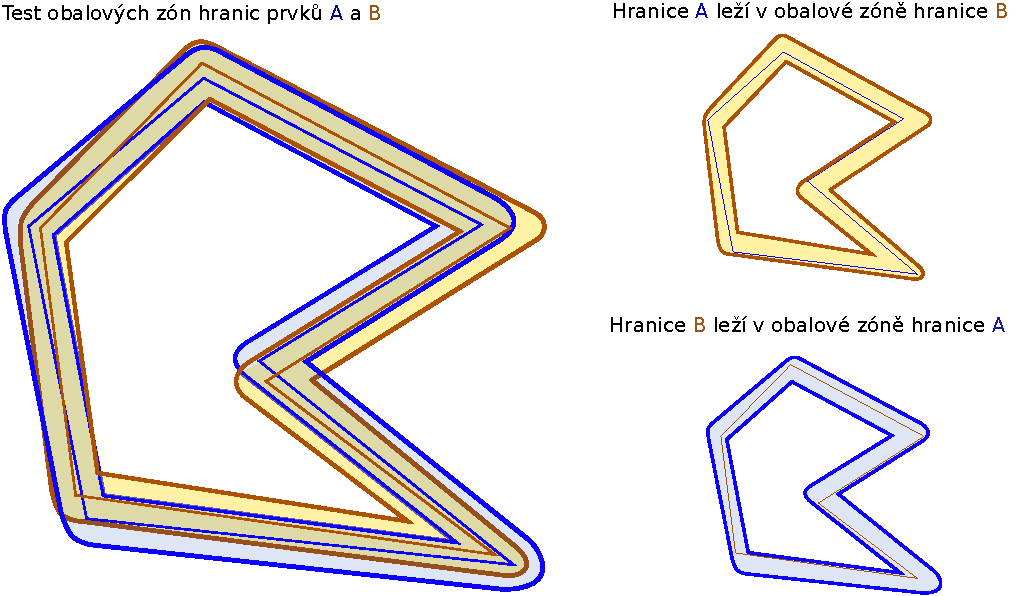
\includegraphics[width=300pt]{./pictures/buffer-boundary.pdf}
      \caption{Porovnání prvků na základě obalových zón jejich hranic(\todo{zdroj})}
      \label{fig:buffer-boundary}
  \end{figure}

\end{enumerate}

%% ML: doplnit ilustraci .. obrázek obal. zón




\subsection{Implementace} % text asi přepsat 
\label{ca-implementace}
% popis mé implementace algoritmu + zmínit třídy a funkce s odkazy na literaturu
Veškeré zpracování je opět schováno pod jedinou funkcí \texttt{align} třídy
\texttt{Coverage\-Alignment}. Ta postupně volá metody provádějící jednotlivé
kroky algoritmu.

Nejdříve je třeba nalézt odpovídající si prvky. K~tomu slouží třída 
\texttt{Matching\-Geometry}, která k~dané geometrii najde odpovídající
(\texttt{set\-Match}). Obdobně jako u~\texttt{Vertex\-Snapper} je i~zde 
využito prostorových indexů, které jsou vytvořeny metodou 
\texttt{build\-Index}. Určení blízkých bodů je pak provedeno prostřednictvím
funkcí \texttt{choose\-Matching\-Points, \-find\-Closest\-Points,
\-clean\-Matching\-Points} třídy \texttt{Co\-ve\-ra\-ge\-Align\-ment}.

Třetím krokem je vytvoření TINu metodou \texttt{create\-TIN}, která k~tomu
využívá třídu \texttt{Tri\-an\-gu\-la\-tion}.  

Konečně je provedena postupně transformace všech prvků. Funkce pro
transformaci poskytuje třída \texttt{Affine\-Trans\-for\-mation},
která transformuje prvky na~základě předané geometrie a~triangulační
sítě. Ta je volána prostřednictvím třídy pro editaci 
\texttt{Align\-Geo\-metry\-Edi\-tor\-Ope\-ra\-tion}.


\subsection{Využití}
\label{ca-vyuziti}

Na~rozdíl od~předchozího algoritmu je tento trochu šířeji využitelný. Je opět 
vhodný pro~zpřesnění vrstvy dle vrstvy referenční, avšak tentokrát nejsou 
pouze přichytávány blízké vrcholy, ale jsou upravovány téměř všechny vrcholy. 
To zajišťuje reálnější výsledky i~v situacích, kdy hustota vrcholů v~obou 
datasetech je velmi rozdílná.

% poznámka o výhodách a nevýhodách využití u liniových a polygon. datech
